\chapter{Transformationen}

\section{Die Hough-Transformation}

Die Hough-Transformation wird verwendet, um Geraden in Bildern zu erkennen. Jede Gerade in einem 
Bild lässt sich eindeutig durch zwei Parameter codieren:
\begin{itemize}
\item Die Richtung der Gerade. Wir suchen dazu nach einem Normalenvektor auf dem Einheitskreis, 
  welcher senkrecht auf die Gerade steht. Jeden Normalenvektor kann man schreiben als
  \[
    v_{\theta} = \begin{pmatrix} \cos(\theta) \\ \sin(\theta) \end{pmatrix},
  \]
  d.h.\ $ \theta $ gibt den Winkel zwischen der $ x $-Achse und dem Vektor $ v_{\theta} $ an. Da es
  zu jeder Gerade offensichtlich zwei Normalenvektoren gibt, beschränken wir uns auf
  $ \theta \in [-\pi / 2, \pi / 2) $, um eine eindeutige Darstellung zu erhalten.
\item Der Abstand $ c \in \R $ der Gerade zum Ursprung. Damit ist die Länge der Strecke gemeint, 
  die durch den Ursprung geht und die Gerade senkrecht schneidet.
\end{itemize}
Die Parametrisierung aller Geraden durch einen Punkt $ x $ des Bildes ist dann gegeben durch
\[
  H(x) = \left\{ 
    (\theta, c) : v_{\theta}^{\top} x = c
  \right\} \subset \left[ -\frac{\pi}{2}, \frac{\pi}{2} \right) \times \R \eqqcolon \mathbb{H}.
\]
Wir betrachten nun eine Menge $ X \subset \R^{2} $ von Punkten (z.B.\ ein Bild) und bilden zu jedem 
der Punkte $ x $ in $ X $ die Menge $ H(x) $. Wir zählen nun, wie oft ein Paar $ (\theta, c) $
insgesamt in den Mengen $ H(x) $ aufgetaucht ist, d.h.\
\[
  n_{X}(\theta, c) \coloneqq \#\{ x \in X : (\theta, c) \in H(x) \}.
\]
Nimmt $ n_{X}(\theta, c) $ einen großen Wert an, dann bedeutet dies, dass wir viele Punkte gefunden
haben, die in einer Linie liegen, sprich eine Gerade bilden. Uns interessiert dabei nicht, welchen
Farb- oder Helligkeitswert die Bildpunkte haben, sondern einfach nur, ob dieser Bildpunkt vorhanden
ist oder nicht. Dazu müssen wir das Bild zuerst binarisieren.

\begin{definition} \leavevmode
\begin{itemize}
\item Ein binarisiertes Bild ist ein Bild, das nur die Werte $ 0 $ oder $ 1 $ annimmt.
  $ 0 $ bedeutet dabei, dass die Farb- oder Grauwertinformation aus dem Originalbild im 
  binarisierten Bild verworfen wird und dieser Bildpunkt im binarisierten Bild \enquote{unsichtbar} 
  sein soll und $ 1 $ bedeutet entsprechend, dass der Bildpunkt aus dem Original auch im 
  binarisierten Bild zu sehen sein soll.
\item Die Hough-Transformation eines endlichen binarisierten Bildes mit Pixeln
  $ X = \{ (x_{j}, y_{j}) \in \R^{2} : j = 1, \ldots, N \} $ ist
  \[
    (H(X))(\theta, c) = n_{X}(\theta, c), \qquad (\theta, c) \in \mathbb{H}.
  \]
\end{itemize}
\end{definition}

Da die meisten Geraden keinen Punkt treffen werden und $ H(X) $ damit fast überall $ 0 $ ist,
zerlegt man $ \mathbb{H} $ normalerweise in kleinere Bereiche $ \mathbb{H}_{jk} $, von denen man
glaubt, dass sie viele Geraden enthalten werden. Dabei ist
$ \mathbb{H}_{jk} \coloneqq \Theta_{j} \times C_{k} $ mit $ j,k = 1, \ldots, M, M' $. $ \Theta_{j} $
ist eine Partition von $ [-\pi / 2, \pi / 2) $ und $ C_{k} $ ist eine Zerlegung eines (hinreichend
großen Teilbereichs) von $ \mathbb{R} $. Damit lässt sich festlegen, in welchen Bereichen des Bildes
man nach welchen Geraden suchen will.

\begin{remark}[Pseudo-Algorithmus zur Diskreten Hough-Transformation] \leavevmode
\begin{enumerate}
\item Gegeben ist ein (beliebiger) Punkt $ p = (x,y) $ des binarisierten Bildes. Wir wollen 
  feststellen, wie viele Geraden durch $ p $ verlaufen.
\item Initialisiere die Matrix $ \mathbf{H} $ mit $ \mathbf{0}_{M \times M'} $. In dieser Matrix
  wird die Häufigkeit codiert, mit der man für ein gegebenes Paar $ (\theta, c) $ den Punkt $ p $
  des Bildes getroffen hat.
\item Für $ j = 1, \ldots, M $:
  \begin{enumerate}
  \item Wähle einen Mittelpunkt $ \theta_{j} $ der Partition $ \Theta_{j} $.
  \item Bestimme einen Index $ k $ mit $ 1 \leq k \leq M' $ so, dass
    \[
      x \cos(\theta_{j}) + y \cos(\theta_{j}) \in C_{k}.
    \]
    D.h., bestimme die Teilbereiche $ C_{k} $ von $ \R $, durch die die Gerade verläuft.
  \item Erhöhe die Anzahl für das entsprechende Paar $ (\theta_{j}, k) $ in der Matrix
  $ \mathbf{H} $ um 1: $ H_{jk} \leftarrow H_{jk} + 1 $.
  \end{enumerate}
\item Ergebnis: $ \mathbf{H} $ ist die diskrete Hough-Transformation.
\end{enumerate}
\end{remark}

Die Matrix $ \mathbf{H} $ kann man nun wiederum als Bild darstellen, indem man die Einträge der
Matrix (die ja Häufigkeiten sind) einfach als Helligkeitswert interpretiert. Die $ x $-Achse des
Bildes gibt den Winkel $ \theta $ der Gerade an, und die $ y $-Achse den Abstand $ c $ der Geraden 
zum Nullpunkt. Ist das Bild an einer Stelle $ (\theta, c) $ hell, so wissen wir, dass die durch
$ (\theta, c) $ codierte Gerade mit hoher Wahrscheinlichkeit eine Gerade in unserem Ursprungsbild
darstellt. Eine andere Möglichkeit, die Ergebnisse der Hough-Transformation zu veranschaulichen,
wäre ein Histogramm zu erstellen, bei dem nach rechts z.B.\ alle Möglichen Paare an Winkel und
Abstand aufgetragen werden und nach oben die Zahl der Punkte, durch die diese Geraden gehen.

\begin{remark}[Vor- und Nachteile der Hough-Transformation] \leavevmode
\begin{itemize}
\item Es werden Kanten erkannt, die in den meisten Fällen eigentlich gar keine Kanten sind, z.B.\ 
  die Ränder des Bildes. Dieser Fehler ist aber leicht zu korrigieren.
\item Die Kanten werden nicht lokalisiert. Wir wissen zwar, durch welche Punkte eine Kante im
  Originalbild verläuft. Wir wissen aber nicht, wo eine Kante tatsächlich beginnt und wo sie endet.
  Dies kann auch ein Vorteil sein, da man so z.B.\ verdeckte Kanten wieder rekonstruieren kann.
\item Bevor die Hough-Transformation auf ein Bild angewendet werden kann, muss dieses binarisiert
  werden. D.h.\ es muss festgelegt werden, welche Pixel des Bildes als potentielle Kanten
  betrachtet werden und welche nicht. Dies geschieht meistens durch Schwellwerte, welche aber durch
  Willkür oder Ausprobieren zustande kommen.
\item Mithilfe der Hough-Transformation lassen sich nicht nur Geraden finden, sondern theoretisch
  alle Kurven, die man irgendwie parametrisieren kann. Z.B.\ kann man Kreise eindeutig durch
  einen Mittelpunkt und Radius darstellen und dies ermöglicht es, mit der Hough-Transformation 
  Kreise im Bild zu finden. Das Problem dabei ist nur, dass mit steigender Zahl an Freiheitsgraden 
  der Aufwand der Transformation \emph{exponentiell} steigt. Je komplexer also die Formen sind,
  nach denen man sucht, desto länger dauert die Transformation. In solchen Fällen hilft es dann nur,
  einen oder mehrere der Freiheitsgrade zu eliminieren, indem man z.B.\ für Kreise einen festen
  Radius oder Mittelpunkt einstellt.
\end{itemize}
Summa summarum: Die Hough-Transformation ist vor allem dann nützlich, wenn man unterbrochene
Kanten im Bild finden will oder das Bild nur durch wenige Kanten dominiert wird.
\end{remark}

\section{Zeit-/Frequenz -- Fenster \& Gabor}

Mit der Fourier-Transformation kann man zwar die in einem Signal enthaltenen Frequenzen analysieren.
Man kann damit aber nicht feststellen, zu welchem Zeitpunkt bzw.\ an welchem Ort des Signals
welche Frequenz auftritt. Ein weiteres Problem besteht in der Fourier-Transformation sehr langer
Signale, was oft die Kapazitäten kleiner Prozessoren in Handys usw.\ übersteigt.

Dies motiviert die Einführung der \emph{Gabor-Transformation}, einer Variante der 
Fourier-Transformation, bei der das Signal in kleineren Stücken durch ein wanderndes 
\enquote{Fenster} betrachtet wird. Denn wenn man die Daten \enquote{fenstert} und nur auf diesem 
Bereich betrachtet, dann sieht man i.W.\ auch nur die Frequenzen, die in diesem Bereich auftreten
und erreicht somit eine bessere Lokalisierung als bei der Fourier-Transformation. Daher wird die 
Gabor-Transformation auch als \enquote{gefensterte Fourier-Transformation} bezeichnet.

\begin{definition}\leavevmode
\begin{itemize}
\item Als \emph{Fensterfunktion} bezeichnen wir eine reelle, gerade und energienormierte Funktion
  $ g $, d.h. $ g(x) = g(-x) $ und $ \norm{g}_{2} = 1 $.
\item Wir definieren
  \[
    \phi_{t, \xi}(x) \coloneqq e^{i\xi x} g(x - t), \qquad x \in \R, \quad (t, \xi) \in \R^{2}.
  \]
\item Die Gabor-Transformation zu einer Funktion $ f $ ist dann definiert als
  \[
      Gf(t,\xi)
    = \langle f, \phi_{t,\xi} \rangle
    = \int_{\R} f(x) \overline{\phi_{t, \xi}}(x) \dif x
    = \int_{\R} f(x) e^{-i \xi x} g(x - t) \dif x,
      \qquad (t, \xi) \in \R^{2}.
  \]
\end{itemize}
\end{definition}

\begin{remark}
Die Gabor-Transformation liefert also ein Spektogramm $ |Gf| : \R^{2} \rightarrow \R $, das angibt,
wieviel Energie sich zu einem bestimmten Zeitpunkt $ t $ in einer bestimmten Frequenz $ \xi $
konzentriert. Natürlich wird das Spektogramm auch beeinflusst durch die Wahl der Fensterfunktion
$ g $. Wählt man z.B.\ die Rechtecksfunktion, so hat man bedingt durch das Abschneiden wieder mit
Artefakten im Spektogramm zu kämpfen. Wählt man hingegen die Gauß-Funktion, so kann man diesem
Effekt etwas entgegentreten, erhält aber dafür ein Fenster, das \enquote{zu den Rändern} hin immer
milchiger wird. Ein weiterer wichtiger Aspekt ist, dass die Länge des Fensters mit der Periodenlänge
des Signals und der Abtastfrequenz kompatibel sein muss. Sonst kommt es zum sog.\ \enquote{Leck-
Effekt}, bei dem Frequenzen im Spektogramm \enquote{verschmiert} werden.
\end{remark}

\begin{proposition}
Für $ f \in L_{2}(\R) $ gilt:
\begin{description}
\item [Inverse Gabor-Transformation]
  \[
    f(x) = \frac{1}{2\pi} \int_{\R} \int_{\R} Gf(t,\xi) e^{i \xi x} g(x - t) \dif \xi \dif t.
  \]
\item [Parseval-Plancherel]
  \[
    \int_{\R} |f(x)|^{2} \dif x = \frac{1}{2\pi} \int_{\R}\int_{\R} |Gf(t,\xi)|^{2} \dif \xi \dif t.
  \]
  Die Gabor-Transformation auf $ L_{2}(\R) $ im Wesentlichen eine Isometrie.
\end{description}
\end{proposition}

\begin{remark}[Implementierung der Gabor-Transformation]
Unter Verwendung der Identität
\[
    (Gf(\bullet, \xi))^{\wedge}(\omega)
  = \widehat{f}(\omega + \xi)\widehat{g}(\omega)
\]
und damit
\[
    Gf(t, \xi)
  = \left( (Gf(t, \xi))^{\wedge} \right)^{\vee}
  = \left( \widehat{f}(\bullet + \xi) \widehat{g} \right)^{\vee}(t),
\]
kann man die Gabor-Transformation effizient über die FFT implementieren, wenn man $ f $ und $ g $
diskret abtastet.
\end{remark}

Die Gabor-Transformation ist ein Beispiel für die sog.\ \emph{Zeit-Frequenz-Analyse}, bei der man
versucht, die in einem Signal auftretenden Frequenzen zu lokalisieren. Ein weiteres Beispiel ist
Notenschrift, bei der die Form einer Note die zu spielende Dauer und die Lage einer Note die
Tonhöhe, also die Frequenz angibt. Intuitiv müsste man meinen, dass ein kleineres Fenster eine 
bessere Lokalisierung zur Folge hat. Das ist im Grunde genommen auch richtig, aber es gibt gewisse 
\enquote{Grenzen}.

\begin{definition}[Zeit-/Frequenzlokalisierung]
Die \emph{Zeitlokalisierung} einer Funktion $ f \in L_{2}(\R) $ ist als
\[
  \mu = \mu(f) = \frac{1}{\norm{f}_{2}^{2}} \int_{\R} t |f(t)|^{2} \dif t
\]
definiert, die \emph{Frequenzlokalisierung} von $ f $ entsprechend als
\[
    \widehat{\mu} = \widehat{\mu}(f)
  = \frac{1}{\norm{\widehat{f}}_{2}^{2}} \int_{\R} \xi |\widehat{f}(\xi)|^{2} \dif t
  = \frac{1}{2\pi \norm{f}_{2}^{2}} \int_{\R} \xi |\widehat{f}(\xi)|^{2} \dif t.
\]
Die \emph{Zeitvariation} von $ f $ ist definiert als
\[
  \sigma^{2} = \frac{1}{\norm{f}_{2}^{2}} \int_{\R} (t - \mu)^{2} |f(t)|^{2} \dif t
\]
und entsprechend die \emph{Frequenzvariation} als
\[
    \widehat{\sigma}^{2}
  = \frac{1}{2\pi \norm{f}_{2}^{2}} 
      \int_{\R} (\xi - \widehat{\mu})^{2} |\widehat{f}(\xi)|^{2} \dif t.
\]
\end{definition}

\begin{remark}[Heisenberg-Boxen]
Eine Funktion hat also ihren Schwerpunkt in Zeit/Frequenz an der Stelle $ (\mu, \widehat{\mu}) $
und die Variationen $ \sigma^{2} $ und $ \widehat{\sigma}^{2} $ geben an, wie gut lokalisiert oder
konzentriert die Funktion in Zeit und Frequenz um den Schwerpunkt ist. Den Bereich
\[
  H(f) \coloneqq 
    [\mu(f) - \sigma(f), \mu(f) + \sigma(f)] \times
    [\widehat{\mu(f)} - \widehat{\sigma(f)}, \widehat{\mu(f)} + \widehat{\sigma(f)}]
\]
bezeichnet man als \emph{Heisenberg-Box} von $ f $.

\begin{figure}
\centering
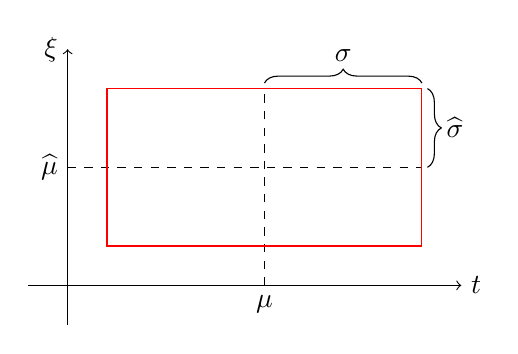
\begin{tikzpicture}
\draw [->] (-0.5,0) -- (5,0) node [right] {$ t $};
\draw [->] (0,-0.5) -- (0,3) node [left] {$ \xi $};
\draw [dashed] (2.5,0) node [below] {$ \mu $} -- (2.5,2.5);
\draw [dashed] (0,1.5) node [left] {$ \widehat{\mu} $} -- (4.5,1.5);
\draw [red] (0.5,0.5) rectangle (4.5,2.5);
\draw [decorate,decoration={brace,mirror,amplitude=5pt},xshift=2pt] 
  (4.5,1.5) -- (4.5,2.5) node [midway,xshift=10pt] { $ \widehat{\sigma} $ };
\draw [decorate,decoration={brace,mirror,amplitude=5pt},yshift=2pt] 
  (4.5,2.5) -- (2.5,2.5) node [midway,yshift=10pt] { $ \sigma $ };
\end{tikzpicture}
\caption{}
\label{fig:Heisenberg-Box}
\end{figure}

\end{remark}